\section{Dataset}\label{section:dataset}

The first part of ISBI Challenge 2017 \cite{codella2018skin} - Skin Lesion Analysis Towards Melanoma Detection: Lesion Segmentation dataset is used in this thesis.
This dataset has train, validation and test data separately.
The training dataset consists of 2000 dermoscopic JPEG images and related masks in PNG format.
The dataset includes various type of lesions such as malignant melanoma, nevus and seborrhoeic keratosis.
Sample images are given with corresponding masks in Figure~\ref{figure:sample-images-from-dataset} where the first row represents original images and second row shows the ground truth aka the corresponding masks.

\begin{figure}
    \centerline{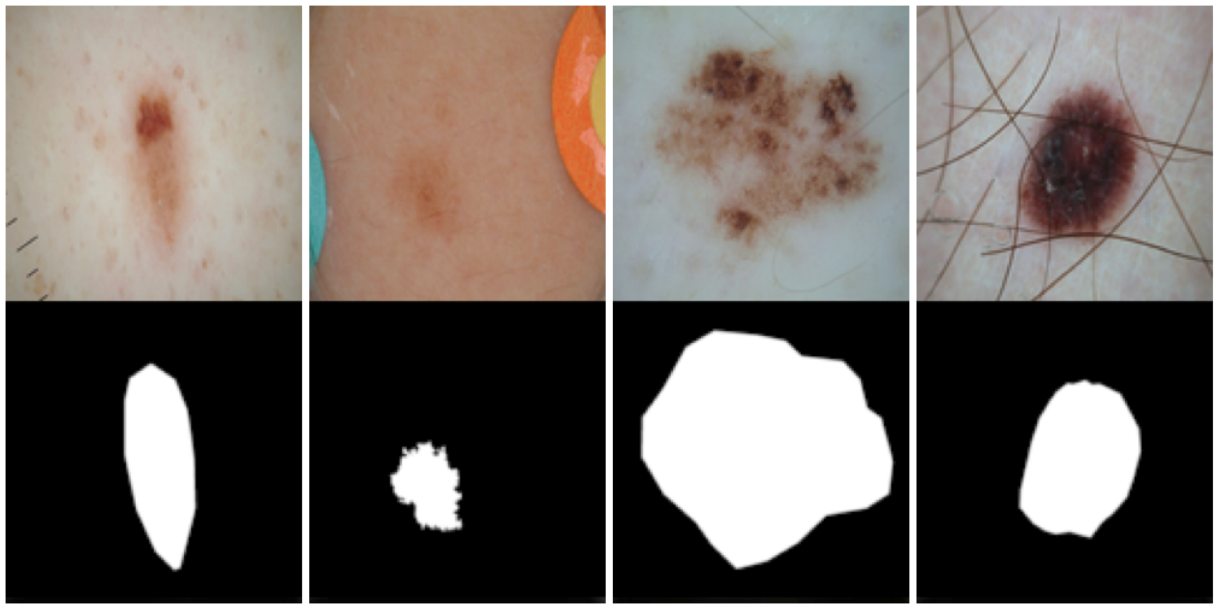
\includegraphics[width=1\columnwidth]{04-methodology/figures/sample-images-from-dataset.png}}
    \caption{Sample images from dataset. First row is original images, second row is corresponding masks}
    \label{figure:sample-images-from-dataset}
\end{figure}

There are also validation and test datasets which contain 150 and 600 images respectively.
The results are based on several common image similarity metrics which are given related section.

\begin{figure}
    \centerline{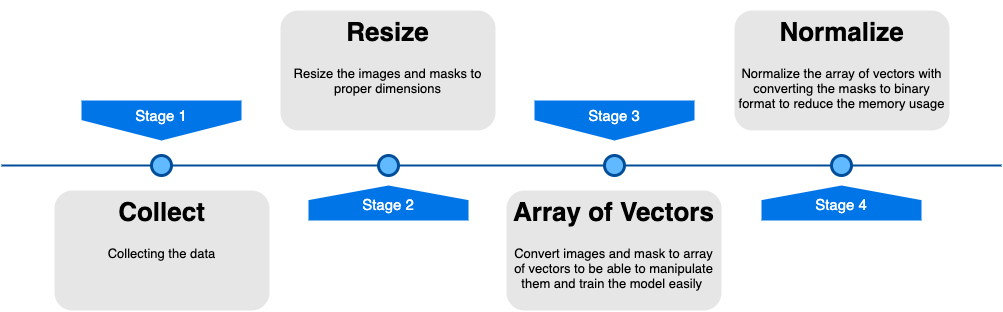
\includegraphics[width=1\columnwidth]{04-methodology/figures/data-preparation-process.png}}
    \caption{Data preparation process}
    \label{figure:data-preparation-process}
\end{figure}

The images are of various dimensions and  neural network model can not handle relatively big images because of the inner constraints in the architecture and memory.
Therefore, all images have been resized into same dimension to reduce the memory consumption and to increase the accuracy as a preprocessing stage.
As it can be stated at Figure~\ref{figure:data-preparation-process}, arrays of mask files have been converted to uint8 to reduce the size of the masks.
